\subsection{Organisation générale}
%schéma tableau

Dans le cadre du projet Simterpose de virtualisation légère et de test
d'applications distribuées, c'est l'émulation par interception qui a été
choisie. En effet, le but final étant de pouvoir évaluer n'importe quelle
application distribuée sur n'importe quel type d'architecture, on peut se
retrouver à devoir émuler des machines plus puissantes que l'hôte, ce que
l'émulation par dégradation ne permet pas. Ce choix exclut donc l'utilisation de
Distem dans notre projet. Les autres outils de virtualisation par interception
ont été écartées pour des raisons différentes: CWRAP utilise uniquement
\texttt{LD\_PRELOAD} pour intercepter les actions et est spécifique aux
applications réseaux. RR gère le multithread mais pas la virtualisation réseau. MicroGrid utilise une émulation par dilation pour gérer le temps. Or, dans notre cas, nous voulons faire de l'interception.

Pour satisfaire les besoins de notre projet, il a été décidé de créer un nouvel
émulateur Simterpose. Ce dernier doit être simple d'utilisation et facilement
déployable (simple ordinateur ou cluster).  De plus, il doit permettre
d'exécuter plusieurs instances d'une application sur une même machine et de proposer une large gamme de conditions d'exécutions (simple n\oe ud ou réseau
complexe). Les expériences devant être reproductibles, l'émulateur doit pouvoir
générer des traces pour les rejouer dans le simulateur. La résistance aux
pannes, et le fait de pouvoir fonctionner sans avoir accès au fichier source de
l'application sont également des conditions à satisfaire.

Simterpose utilise la plateforme de simulation SimGrid, dont l'architecture
est représentée (Figure \ref{SimGrid}), pour générer l'environnement virtuel
nécessaire à l'expérience. À sa création en 1999, SimGrid
\citep{CASANOVA:SimGrid} était une plateforme fournissant des outils pour
construire un simulateur afin d'étudier les algorithmes d'ordonnancement en
environnement hétérogène, puis il a évolué \citep{MARTIN:SimGrid} pour devenir
plus générique. Aujourd'hui, c'est devenu une plateforme de simulation
permettant d'évaluer les applications distribuées large échelle s'exécutant dans
des environnements hétérogènes.
 
\begin{figure}[H]
  \centering
  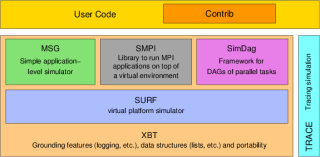
\includegraphics[scale=0.86]{Pictures/png/SimGrid}
  \caption{Architecture de la plateforme SimGrid.}
  \label{SimGrid}
\end{figure}

La Figure \ref{Organisation_generale} présente l'organisation générale de la plateforme de simulation. SimGrid va générer l'environnement virtuel. Simterpose intercepte les
actions de l'application et les modifie pour maintenir l'émulation si
nécessaire. Puis, il les laisse
s'exécuter sur la machinie hôte et va interroger SimGrid pour qu'il calcule la
réponse de l'environnement virtuel aux actions de l'application (temps d'exécution, gestion de communications réseaux). La Figure \ref{Organisation_Simterpose} illustre ce fonctionnement.

\begin{figure}[H]
  \centering
  %\includesvg{Pictures/svg/Communications_Simterpose_interprocess_v2}
  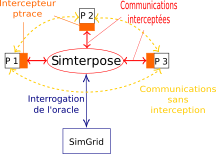
\includegraphics{Pictures/png/Communications_Simterpose_interprocess_v2}
  \caption{Architecture de communication entre les différents acteurs.}
  \label{Organisation_generale}
\end{figure}

\begin{figure}[H]
  \centering
  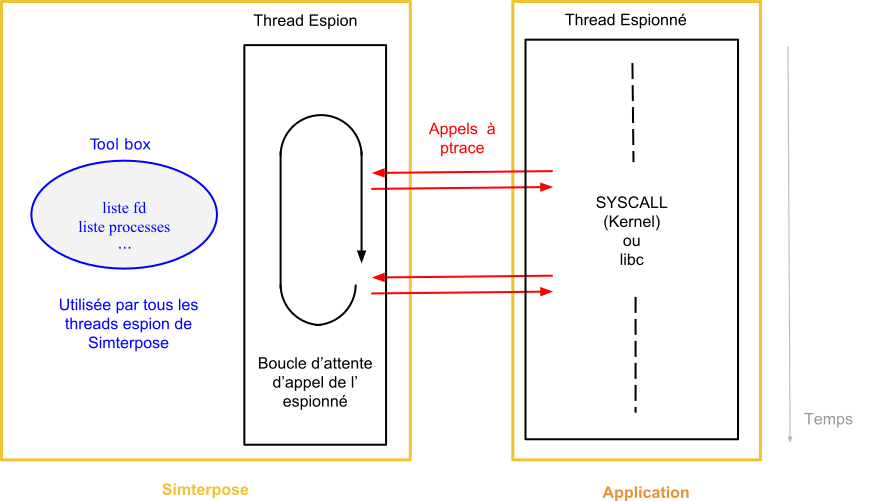
\includegraphics[scale=0.5]{Pictures/png/Simterpose_orga_code_v3}
  \caption{Le fonctionnement de Simterpose.}
  \label{Organisation_Simterpose}
\end{figure}

Maintenant que nous avons présenté le cadre général et l'organisation globale
de notre projet, nous allons nous intéresser au fonctionnement de Simterpose.
